\documentclass[11pt]{article}

\usepackage[margin=1in]{geometry}
\usepackage[T1]{fontenc}
\usepackage{lmodern}
\usepackage{microtype}
\usepackage{booktabs}
\usepackage{array}
\usepackage{siunitx}
\usepackage{graphicx}
\usepackage{xcolor}
\usepackage{hyperref}
\usepackage{caption}
\usepackage{subcaption}
\usepackage{float}
\usepackage{tikz}
\usepackage{pgfplots}
\usepackage{pgfplotstable}

\pgfplotsset{compat=1.18}
\usetikzlibrary{arrows.meta, positioning, shapes.geometric, fit}
\usepgfplotslibrary{groupplots}
\sisetup{
  round-mode=places,
  round-precision=3,
  detect-all
}

\definecolor{coreblue}{HTML}{1F77B4}
\definecolor{socred}{HTML}{D62728}
\definecolor{fpgaorange}{HTML}{FF7F0E}
\definecolor{simgreen}{HTML}{2CA02C}
\definecolor{softgray}{HTML}{666666}

\begin{document}
\begin{titlepage}
    \begin{center}
        \vspace*{2cm}
        \Huge\textbf{Final Architecture Selection} \\
        \vspace{0.25cm}
        \Large\textit{ELEC 5803} \\
        \vspace{2cm}
        \Large Jesse Levine (101185127) \\
        \vfill
    \end{center}
\end{titlepage}

\section{Project Evolution}

This project evolved through five reports that directly informed the final architecture. Report 4 is intentionally omitted here because it did not influence the final design path.

\subsection*{Report 1: Baseline RV32I Build}
Report 1 established the starting point: a reproduced HLS RV32I processor based on a unified memory architecture. The main contribution of that phase was methodological rather than architectural. It demonstrated how bare-metal RISC-V programs could be compiled into hexadecimal memory images, loaded into the HLS model, and evaluated through C/RTL co-simulation. That phase created the baseline measurement framework for clock frequency, cycle count, and functional correctness.

\subsection*{Report 2: Domain Selection and RV32IM Extension}
Report 2 selected machine-learning inference acceleration as the project domain, with SoftMax chosen as the target kernel because of its expensive exponentiation, accumulation, and normalization stages. To make that domain practical on the CPU, the core was extended from RV32I to RV32IM through the introduction of multiplication support. This phase therefore moved the project from ``general processor reproduction'' to ``domain-capable processor baseline''.

\subsection*{Report 3: SoftMax Accelerator Proposal}
Report 3 proposed the specialization strategy that ultimately became the final architecture. The key design decisions were already visible at this point: a memory-mapped accelerator, shared memory between processor and accelerator, approximate exponentiation through LUT/PLA methods, and a pipelined hardware path for reduction and normalization. This report defined the architectural thesis that the rest of the project validated.

\subsection*{Report 5: Pipelined Core and Initial Accelerator}
Report 5 delivered the first meaningful performance comparison. The RV32IM core was pipelined, and a first standalone SoftMax accelerator was implemented and benchmarked. That report showed two critical results: the software SoftMax running on the core scaled linearly but with a very high per-element cost, and the dedicated accelerator reduced latency dramatically while also preserving the SoftMax sum much more accurately as $N$ increased.

\subsection*{Report 6: Final Accelerator and SoC Integration}
Report 6 transformed the standalone accelerator into a complete system by integrating it with the processor as a memory-mapped peripheral inside the Prometheus\_SoC. The architecture used shared BRAM, a Zynq-based control plane, and MMIO control registers so the CPU could configure the accelerator and then read results back from the same memory space. That report established the final design direction: the selected architecture was no longer ``core only'' or ``accelerator only,'' but a complete core-plus-accelerator SoC.

\section{Final Architecture Selection}

The selected final architecture is the integrated Prometheus\_SoC: a RISC-V core combined with a dedicated SoftMax accelerator, implemented as a shared-memory, MMIO-controlled subsystem and deployed on the PYNQ-Z1.

The architectural decision is justified by two observations. First, the software-only core is instruction-bound; the entire SoftMax computation must be emulated through sequential fixed-point arithmetic, causing latency to scale with a large per-element cost and causing the normalization sum to degrade significantly as $N$ grows. Second, the integrated SoC offloads the expensive numerical work into specialized hardware that exploits pipelining, SIMD-style memory access, and dedicated arithmetic structures. This reduces the per-element cost to less than one clock cycle in the final integrated measurements and preserves the SoftMax sum near unity across the full tested range.

\begin{figure}[ht]
\centering
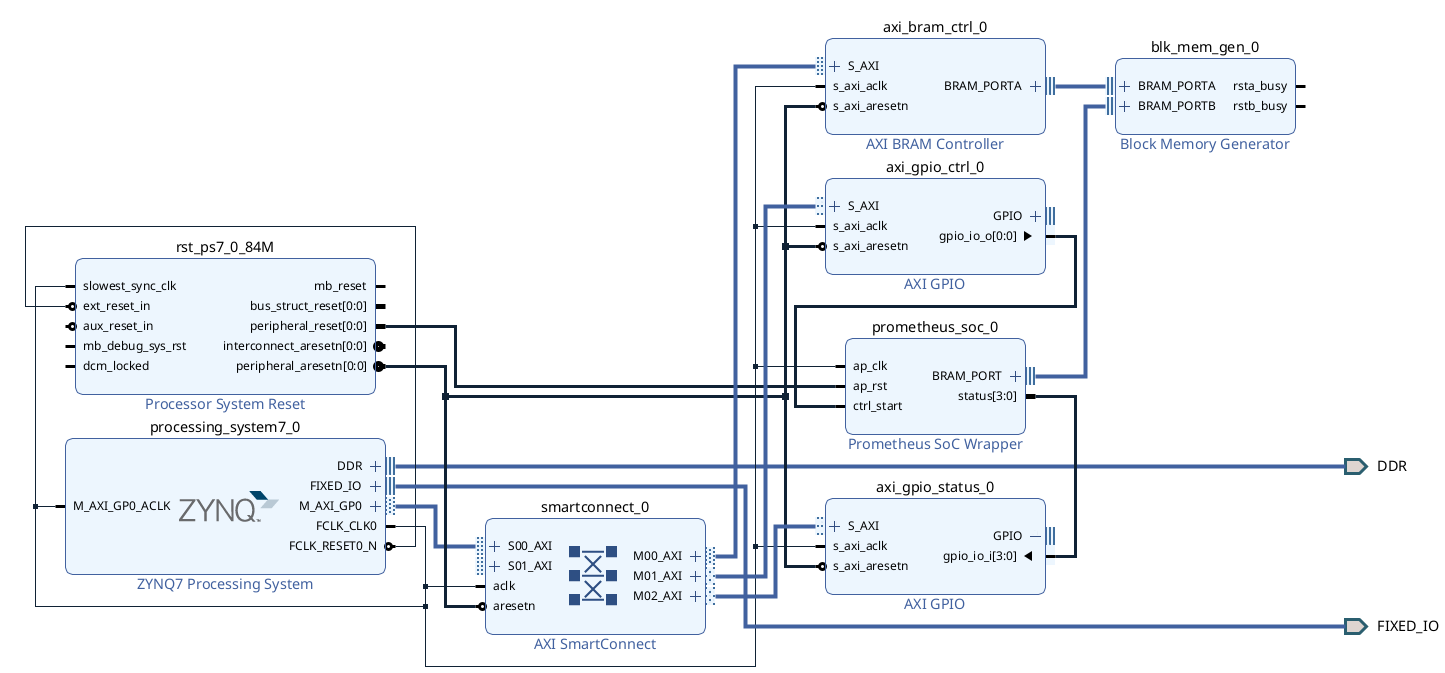
\includegraphics[width=0.95\textwidth]{figures/report6-000.png}
\caption{Vivado block diagram of the implemented Prometheus\_SoC on the PYNQ-Z1, reused from Report 6. The figure shows the Zynq processing system, AXI SmartConnect, AXI BRAM controller, GPIO control/status path, shared BRAM, and the packaged Prometheus\_SoC wrapper.}
\end{figure}

Figure~1 shows the actual Vivado block design used for deployment on the PYNQ-Z1. The Zynq processing system acts as the host-side controller and provides the AXI master interface, clocking, and reset distribution for the programmable logic. Through the AXI SmartConnect, the processing system can access the BRAM controller and the GPIO peripherals that expose the SoC control and status path. The shared BRAM is the central storage element of the design: it holds the RISC-V program image, the input logits, the output probability vector, and the debug values read back after execution.

The packaged Prometheus\_SoC wrapper contains the RISC-V core together with the integrated SoftMax accelerator. From the software point of view, the accelerator is invoked through memory-mapped registers, so the CPU can write the input base address, output base address, debug base address, and vector length before asserting the start signal. From the hardware point of view, both the core and the accelerator operate over the same BRAM address space, which avoids explicit data copying or DMA movement. This is the key systems insight of the final architecture: the CPU remains responsible for orchestration and control flow, while the accelerator is tightly integrated into the same memory system and handles the computationally intensive SoftMax computation directly.

\section{Core-Only vs. Core + Accelerator SoC}

The core-versus-SoC comparison is based on the implementation-level datasets developed in the earlier reports. This is the correct comparison space for architecture selection because it compares the software-only baseline against the final integrated architecture without introducing the separate timing-closure issue of the standalone FPGA baseline wrapper.

\subsection{Implementation Summary}

\begin{table}[ht]
\centering
\caption{Implementation-level resource summary used for architectural comparison. The baseline core values come from the pipelined RV32IM implementation flow, while the SoC values come from the Prometheus\_SoC Vivado IP-flow implementation.}
\label{tab:impl_compare}
\begin{tabular}{lcc}
\toprule
Resource / Metric & Core Only & Core + Accelerator SoC \\
\midrule
LUT & 2169 & 26090 \\
FF & 1465 & 52339 \\
DSP & 12 & 32 \\
BRAM & 0 & 9 \\
Post-route period (ns) & 11.345 & 11.514 \\
\bottomrule
\end{tabular}
\end{table}

The area increase is expected: the final SoC includes not only the CPU but also the complete SoftMax accelerator datapath, additional buffering, and the memory-mapped control structure needed for hardware-software interaction. The architectural question is therefore whether the added area is justified by the latency and numerical gains. Figures~\ref{fig:latency_compare}--\ref{fig:speedup_compare} show that it is.

\subsection{Latency, Numerical Stability, and Speedup}

\begin{figure}[ht]
\centering
\begin{subfigure}[t]{0.48\textwidth}
\centering
\begin{tikzpicture}
\begin{groupplot}[
    group style={group size=1 by 2, vertical sep=1.2cm},
    width=0.95\linewidth,
    height=4.9cm,
    xlabel={Sequence length $N$},
    grid=both,
    grid style={gray!20},
    tick label style={font=\small},
    label style={font=\small}
]
\nextgroupplot[
    ylabel={Core cycles},
]
\addplot+[black, mark=*, thick] table[x=n, y=core_cycles, col sep=comma] {data/core_vs_soc.csv};
\nextgroupplot[
    ylabel={SoC cycles},
]
\addplot+[black, mark=square*, thick] table[x=n, y=soc_cycles_sim, col sep=comma] {data/core_vs_soc.csv};
\end{groupplot}
\end{tikzpicture}
\caption{Latency scaling on separate axes, since a shared axis hides the SoC behavior.}
\end{subfigure}
\hfill
\begin{subfigure}[t]{0.48\textwidth}
\centering
\begin{tikzpicture}
\begin{axis}[
    width=\linewidth,
    height=6.2cm,
    xlabel={Sequence length $N$},
    ylabel={SoftMax sum},
    ymin=0.64,
    ymax=1.02,
    grid=both,
    grid style={gray!20},
    legend style={at={(0.02,0.98)}, anchor=north west, draw=none, fill=none, font=\small},
    tick label style={font=\small},
    label style={font=\small}
]
\addplot+[color=coreblue, only marks, mark=*, mark size=2.0pt] table[x=n, y=core_sum, col sep=comma] {data/core_vs_soc.csv};
\addlegendentry{Core only}
\addplot+[color=socred, only marks, mark=square*, mark size=2.0pt] table[x=n, y=soc_sum_sim, col sep=comma] {data/core_vs_soc.csv};
\addlegendentry{Core + accelerator SoC}
\addplot[dashed, color=softgray] coordinates {(0,1) (140,1)};
\end{axis}
\end{tikzpicture}
\caption{Normalization comparison between the software-only core and the integrated SoC.}
\end{subfigure}
\caption{Implementation-level comparison between the software SoftMax running on the pipelined core and the final integrated Prometheus\_SoC.}
\label{fig:latency_compare}
\end{figure}

\begin{figure}[ht]
\centering
\begin{tikzpicture}
\begin{axis}[
    width=0.72\textwidth,
    height=6.5cm,
    xlabel={Sequence length $N$},
    ylabel={Speedup ratio},
    ymin=0,
    ymax=125,
    grid=both,
    grid style={gray!20},
    tick label style={font=\small},
    label style={font=\small},
    legend style={at={(0.02,0.98)}, anchor=north west, draw=none, fill=none, font=\small}
]
\addplot+[black, mark=triangle*, thick] table[x=n, y=speedup, col sep=comma] {data/core_vs_soc.csv};
\addlegendentry{Measured ratio}
\end{axis}
\end{tikzpicture}
\caption{Speedup of the integrated SoC over the software-only core. Based on the linear models from the prior implementation study, the asymptotic maximum speedup is $\frac{287.89}{0.74} \approx 389\times$.}
\label{fig:speedup_compare}
\end{figure}

The architectural conclusion is unambiguous. The core-only implementation exhibits a high per-element cost and significant numerical degradation as the vector length increases. In contrast, the integrated SoC keeps the SoftMax sum extremely close to $1.0$ and reduces cycle count by more than an order of magnitude even at moderate values of $N$. By $N=128$, the measured cycle ratio exceeds $114\times$, while the linear-fit asymptote from the earlier implementation study indicates a theoretical maximum speedup of approximately $389\times$ for sufficiently large $N$.

\section{FPGA Implementation on the PYNQ-Z1}

The final project requirement was not only to select an architecture, but to actually deploy the full SoC to a physical FPGA. That requirement was satisfied by implementing Prometheus\_SoC on the Digilent PYNQ-Z1, which uses the Xilinx Zynq-7020 (\texttt{xc7z020clg400-1}) device.

\subsection{Implemented PYNQ-Z1 SoC Summary}

\begin{table}[ht]
\centering
\caption{Actual PYNQ-Z1 implementation summary for the full Prometheus\_SoC. This table refers to the complete board-integrated design, not only the HLS IP block.}
\label{tab:fpga_soc}
\begin{tabular}{lc}
\toprule
Metric & Implemented SoC on PYNQ-Z1 \\
\midrule
Board & Digilent PYNQ-Z1 \\
FPGA & \texttt{xc7z020clg400-1} \\
Clock period (ns) & 11.875 \\
Clock frequency (MHz) & 84.211 \\
WNS (ns) & 0.332 \\
WHS (ns) & 0.010 \\
Slice LUTs & 32717 \\
Slice Registers & 60358 \\
Block RAM Tiles & 68.5 \\
DSPs & 32 \\
Timing status & Met \\
\bottomrule
\end{tabular}
\end{table}

This final implementation result is significant for two reasons. First, the full system met timing after actual board-level integration, which means the accelerator benefit survives beyond HLS co-simulation and beyond isolated IP export. Second, the design was exercised on the physical PYNQ-Z1 through the Zynq processing system, AXI interconnect, shared BRAM, and the GPIO control/status path used for run-time launch and monitoring.

\subsection{FPGA Verification Against Simulation}
The goal in this section was to show that the \emph{implemented SoC} behaved on the FPGA in the same way as it did in the earlier simulation and implementation studies. 
Table \ref{tab:fpga_verify} provides that evidence directly.

\begin{figure}[H]
\centering
\begin{subfigure}[t]{0.48\textwidth}
\centering
\begin{tikzpicture}
\begin{axis}[
    width=\linewidth,
    height=6.2cm,
    xlabel={Sequence length $N$},
    ylabel={Clock cycles},
    grid=both,
    grid style={gray!20},
    legend style={at={(0.02,0.98)}, anchor=north west, draw=none, fill=none, font=\small},
    tick label style={font=\small},
    label style={font=\small}
]
\addplot+[black, mark=*, thick] table[x=n, y=cycles, col sep=comma] {data/prometheus_soc_n_sweep.csv};
\addlegendentry{FPGA sweep}
\end{axis}
\end{tikzpicture}
\caption{Latency}
\end{subfigure}
\hfill
\begin{subfigure}[t]{0.48\textwidth}
\centering
\begin{tikzpicture}
\begin{axis}[
    width=\linewidth,
    height=6.2cm,
    xlabel={Sequence length $N$},
    ylabel={SoftMax sum},
    ymin=0.998,
    ymax=1.001,
    ytick={0.998,1.000,1.001},
    yticklabel style={/pgf/number format/fixed, /pgf/number format/precision=4},
    grid=both,
    grid style={gray!20},
    tick label style={font=\small},
    label style={font=\small}
]
\addplot+[black, only marks, mark=*, mark size=1.6pt] table[x=n, y=sum, col sep=comma] {data/prometheus_soc_n_sweep.csv};
\addplot[dashed, color=softgray] coordinates {(0,1) (260,1)};
\end{axis}
\end{tikzpicture}
\caption{FPGA normalization behavior}
\end{subfigure}
\caption{Hardware behavior of the implemented Prometheus\_SoC on the PYNQ-Z1 across the full FPGA sweep.}
\label{fig:fpga_validation}
\end{figure}

\begin{table}[H]
\centering
\caption{Selected simulation-versus-FPGA verification points for the implemented SoC.}
\label{tab:fpga_verify}
\begin{tabular}{cccccc}
\toprule
$N$ & Sim cycles & FPGA cycles & Sim sum & FPGA sum & FPGA latency ($\mu$s) \\
\midrule
2   & 229 & 229 & 1.003448 & 1.003448 & 2.719 \\
8   & 232 & 232 & 1.000183 & 1.000183 & 2.755 \\
32  & 250 & 250 & 1.000320 & 1.000320 & 2.969 \\
64  & 274 & 274 & 1.000000 & 1.000000 & 3.254 \\
128 & 322 & 322 & 0.999344 & 0.999344 & 3.824 \\
\bottomrule
\end{tabular}
\end{table}

The FPGA data confirms that the implemented design reproduces the expected system behavior. Across the complete hardware sweep from $N=2$ to $N=256$, the measured SoC latency remained low and scaled gently with vector length, while the SoftMax sum remained near unity. Representative FPGA measurements include $229$ cycles at $N=2$, $274$ cycles at $N=64$, $322$ cycles at $N=128$, and $418$ cycles at $N=256$. At the largest tested vector size, the probability sum remained $0.997955$, which is entirely consistent with fixed-point quantization rather than architectural error. Table~\ref{tab:fpga_verify} shows that the FPGA measurements matched the earlier SoC simulation values almost exactly at the sampled points.

This is the key verification result of the project: the selected architecture was not only attractive in simulation, but also functionally realized on the target FPGA and observed to behave almost exactly as predicted by the earlier studies.

\section{Final Selection}

The final architecture selection is therefore the integrated Prometheus\_SoC. It is the only design in the project that satisfies all of the important objectives simultaneously:

\begin{itemize}
    \item it preserves the RISC-V core as the system controller rather than replacing the processor entirely,
    \item it removes the SoftMax bottleneck through dedicated hardware,
    \item it maintains numerical stability much more effectively than the software-only core,
    \item it meets timing in the final board-level implementation, and
    \item it has been exercised successfully on the actual PYNQ-Z1 FPGA.
\end{itemize}

The software-only core remains important as the historical baseline because it quantifies the bottleneck that motivated the accelerator. However, the final deliverable is not the baseline core. The final deliverable is the verified SoC implementation on FPGA, and the results show that this was the correct architectural end point for the project.

\section{AI Usage}

Codex CLI and ChatGPT were used throughout the final stage of the project. In this deliverable, AI assistance was used to organize the prior report evidence, recover numerical datasets from stored spreadsheets and implementation reports, generate the LaTeX report structure, and prepare native \LaTeX{} plots and tables. AI was also used during the FPGA deployment stage to help construct the JTAG execution flow and validation scripts for the PYNQ-Z1 hardware.

\end{document}
